\section{Requirements}
	\subsection {Guest Requiremets}
		\subsubsection {System Registration}
			The system needs to enable sign up for new users. This will unlock the user, after a login, the access to the advanced features.
			\begin {figure}[h!]
				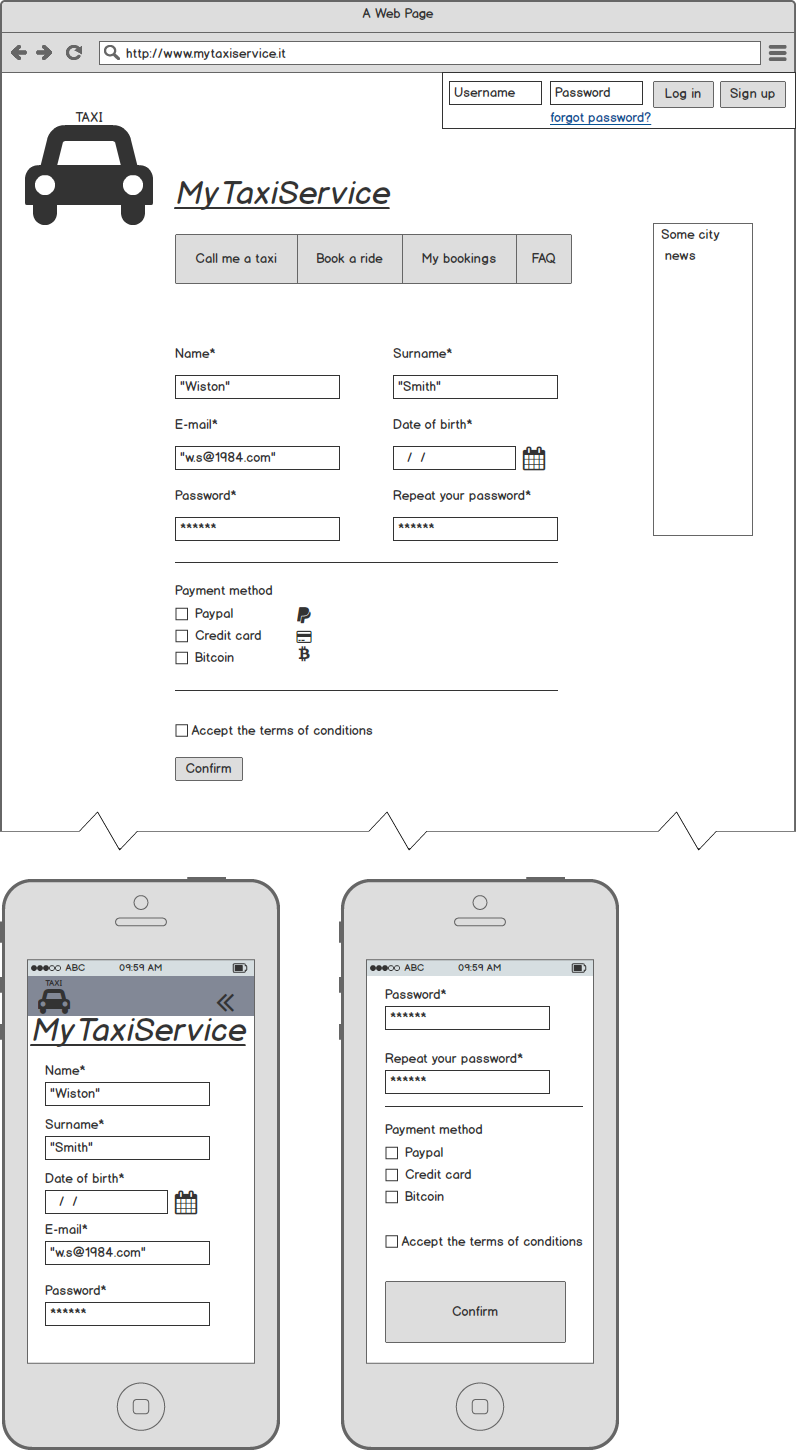
\includegraphics [width=0.6\textwidth, width=6cm]{signup}
				\caption {\askpippo}
			\end {figure}
			\newpage
		\subsubsection {User Login}
		 	The system must provide an authentication system that enable the access to advanced features.
		 	\begin{figure}[h!]
				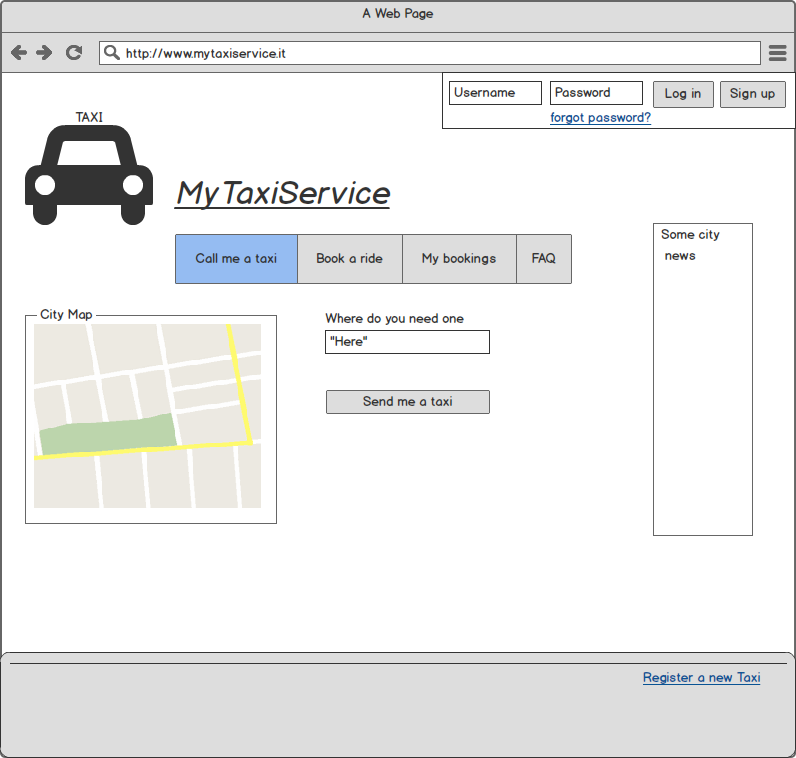
\includegraphics[width=0.6\textwidth]{home}
				\caption{\askpippo.}
			\end{figure}
			\newpage
		\subsubsection {Instant Calls}
			The system must let unregistered user call a taxi immediately.
			\begin{figure}[h!]
				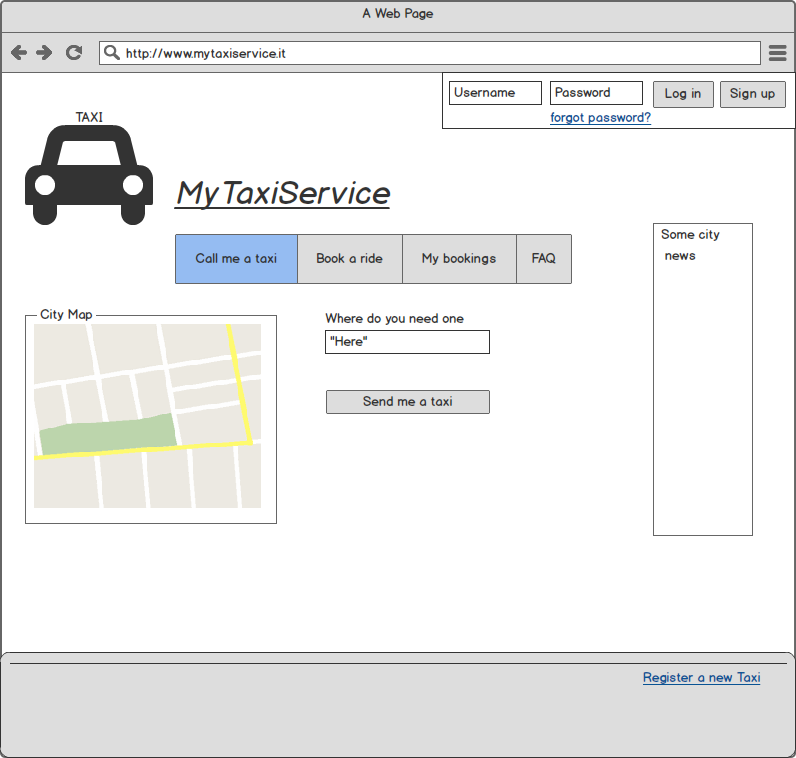
\includegraphics[width=0.6\textwidth]{home}
				\caption{\askpippo.}
			\end{figure}
			\newpage
	\subsection {Registered User Requirements}
		\subsubsection {User edit information}
			The system must have a profile editing function, where a user can change personal data, such as name as well as their address,
			and also add new payment options. On top of that, the system shall log all the rides a user makes into a database.
			\begin{figure}[h!]
				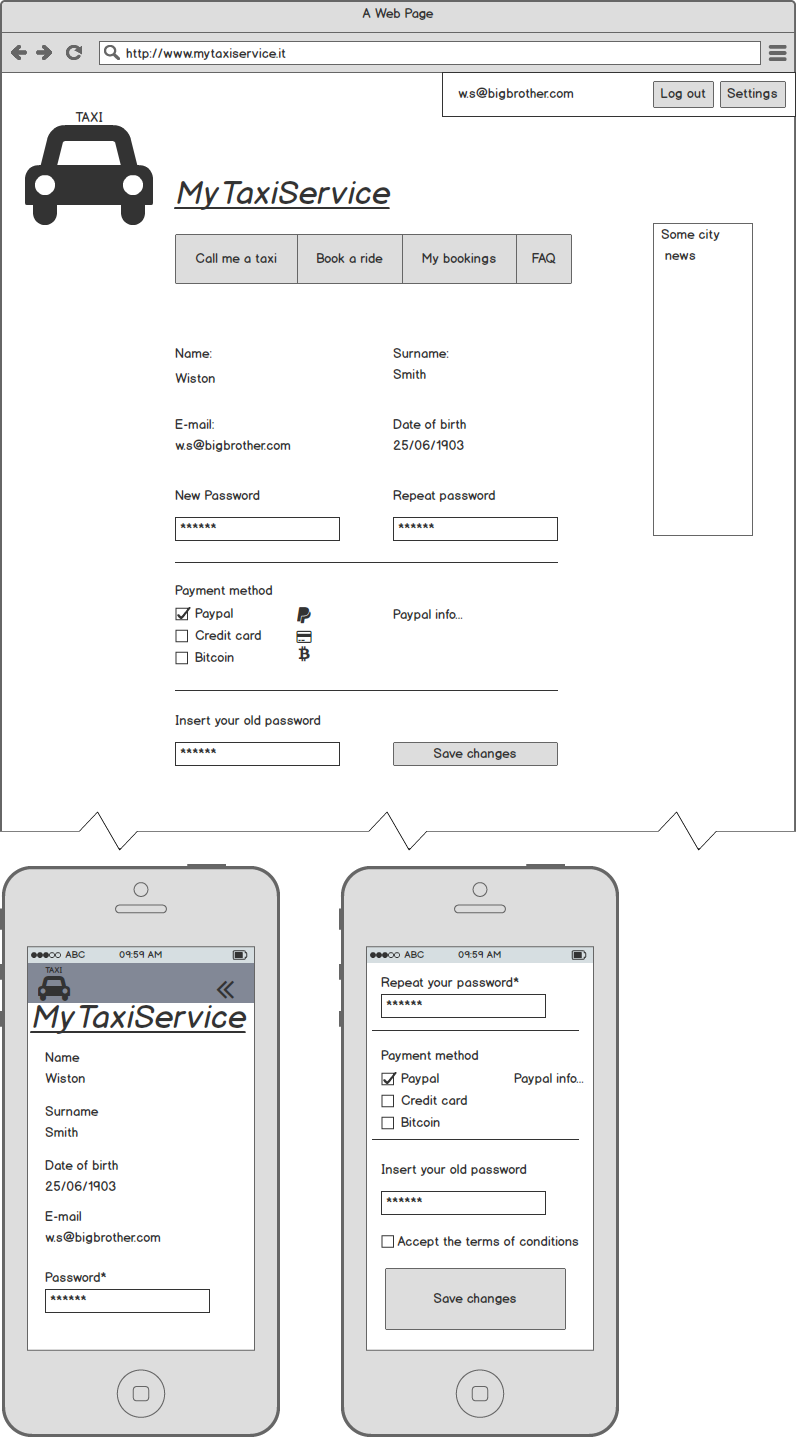
\includegraphics[width=0.6\textwidth]{edituser}
				\caption{Edit form.}
			\end{figure}
			\newpage
		\subsubsection {Instant Calls}
			The system must let registered user call a taxi immediately and give them some advance options.
			\begin{figure}[h!]
				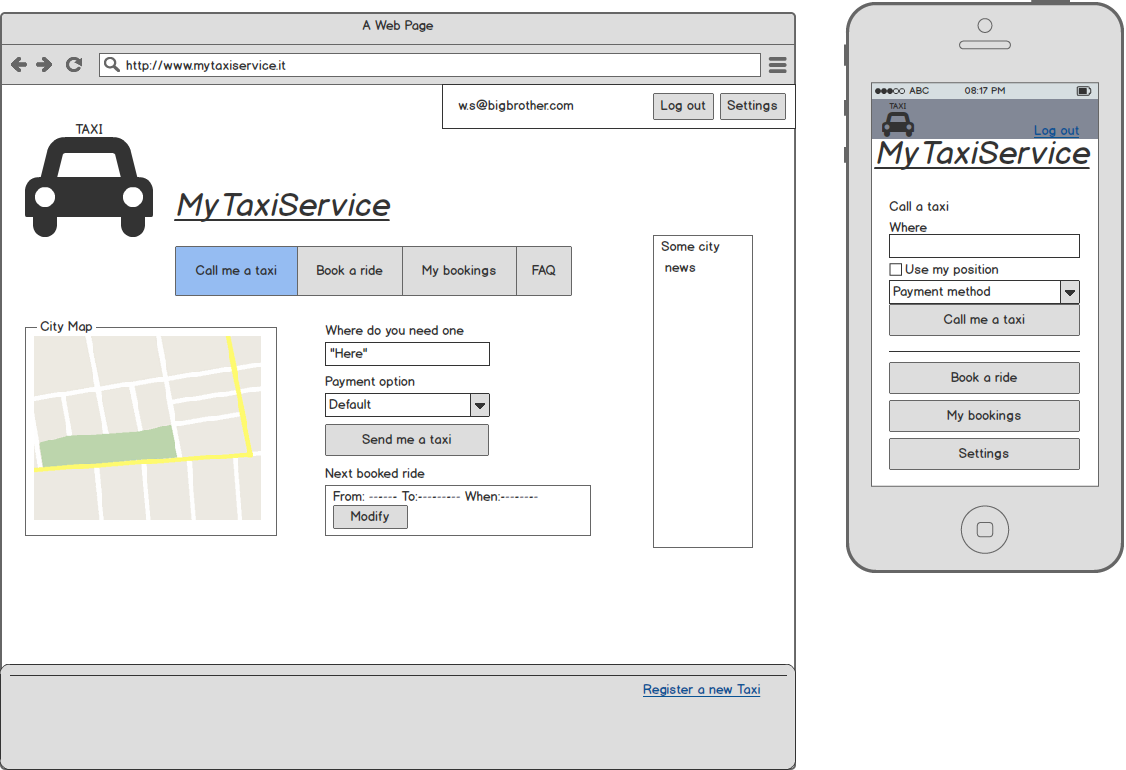
\includegraphics[width=0.6\textwidth]{homelog}
				\caption{Home page of a logged user.}
			\end{figure}
			\newpage
		\subsubsection {Booking and Sharing}
			The system must let registered users book a ride for a specific date and time. On top of that, there has to be an option to share
			rides with other people who are booking similar routes. Notifications must be sent when a match is found for shared rides.
			\begin{figure}[h!]
				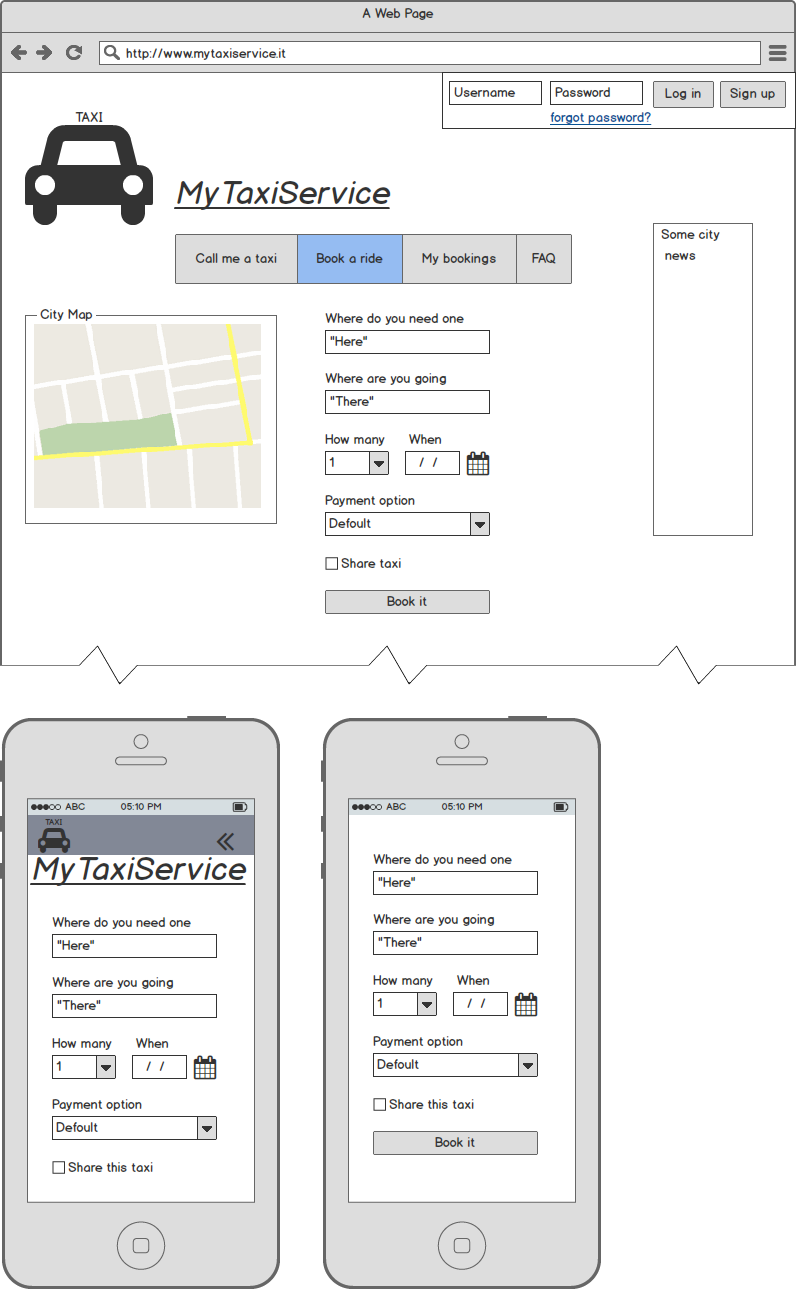
\includegraphics[width=0.6\textwidth]{bookride}
				\caption{Web and app pages used for book a ride.}
			\end{figure}
			\newpage
		\subsubsection {Booking History}
			The system must let the user to see their booking history and let the acces to the editing of a future ride.
			\begin{figure}[h!]
				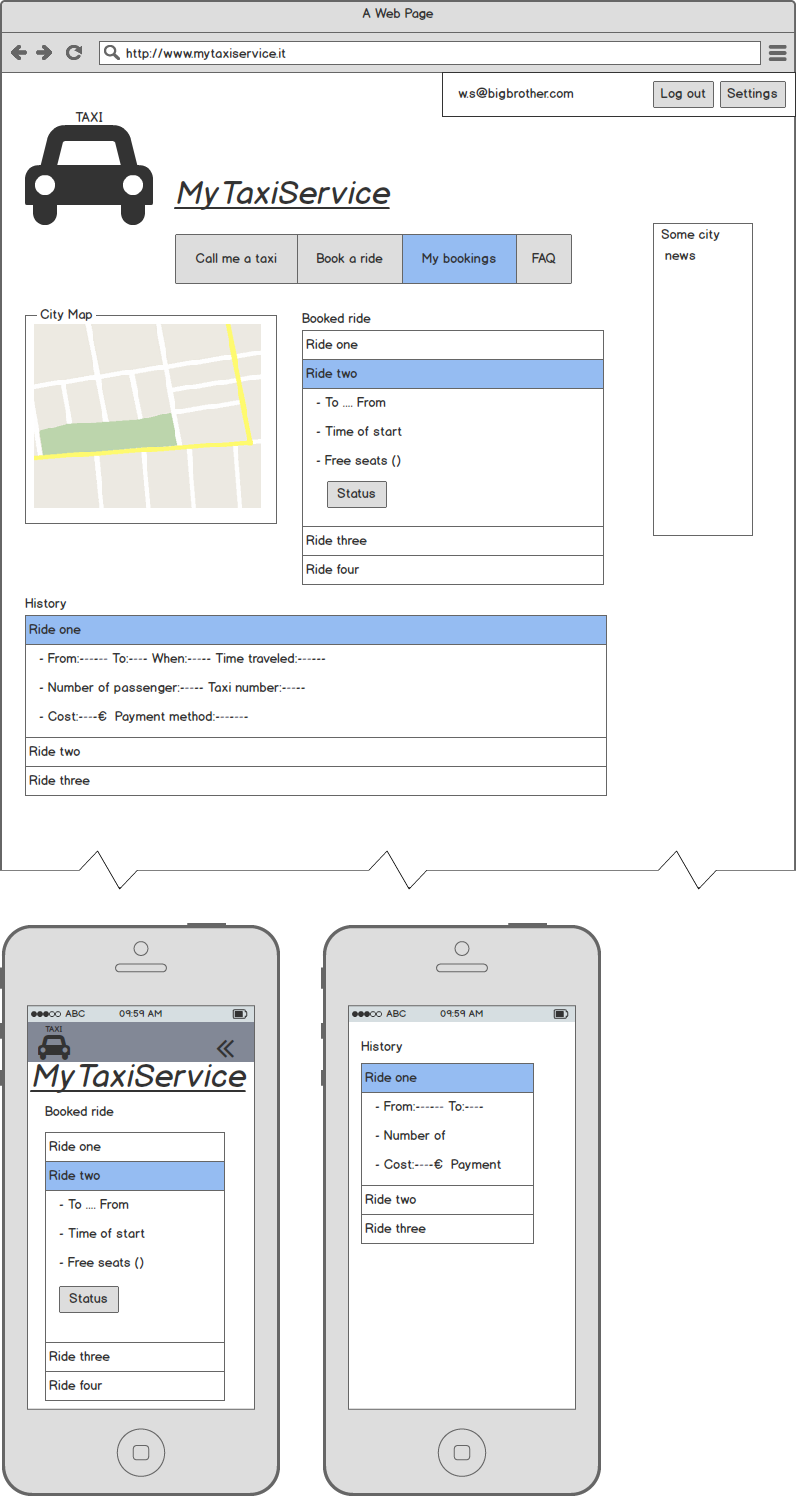
\includegraphics[width=0.6\textwidth]{history}
				\caption{Booked ride history.}
			\end{figure}
		\subsubsection {Booking Editing}
			The system must let the user to modify or cancel a booked ride (if the ride has not been locked).
			\begin{figure}[h!]
				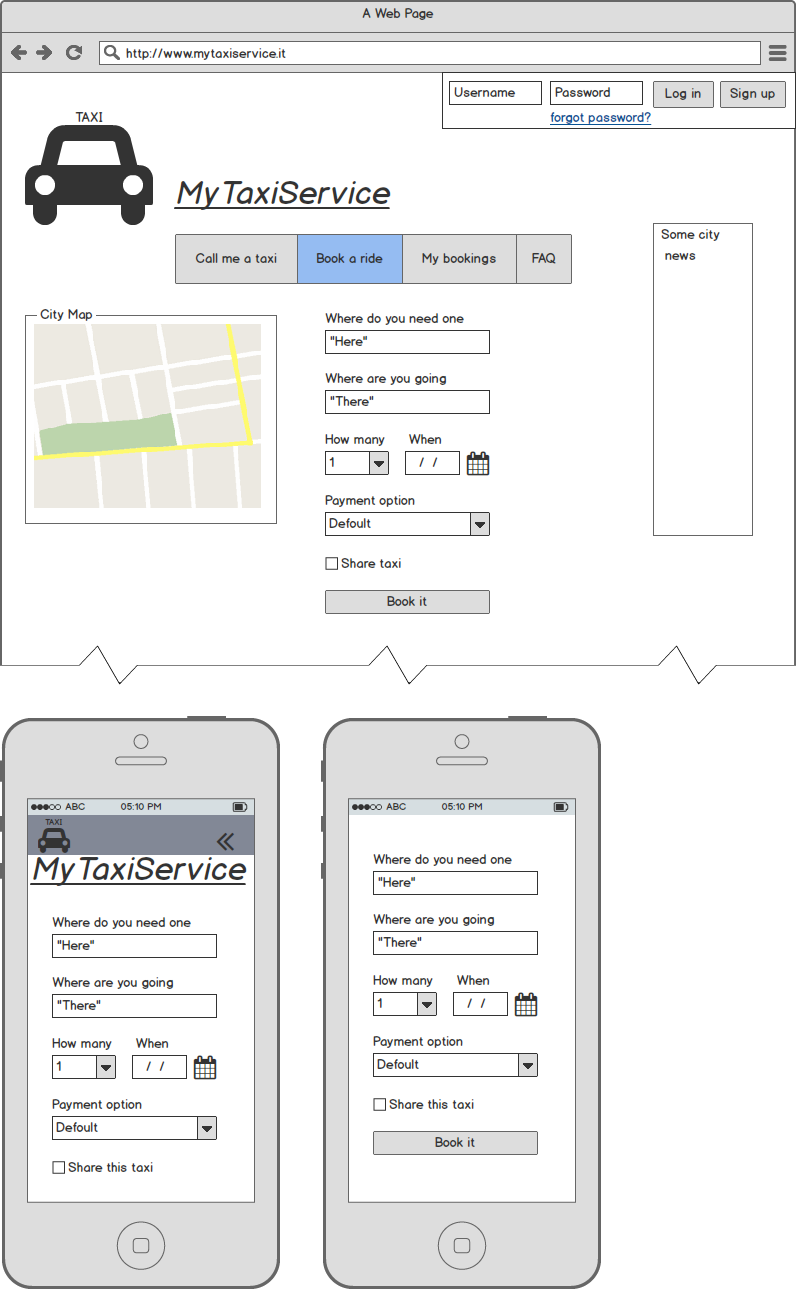
\includegraphics[width=0.6\textwidth]{bookride}
				\caption{Ride editing form.}
			\end{figure}
			\newpage
	\subsection {Taxi Driver Requirements}
		The worker queue must be handled automatically by the system. This includes building a queue dynamically using a FIFO model. The system
		must also provide a mobile app for the driver to get acces to \askpippo
		\subsubsection {Driver Login}
		 	The system must provide a driver's authentication system that enable the driver to acces his feature.
		 	\begin{figure}[h!]
				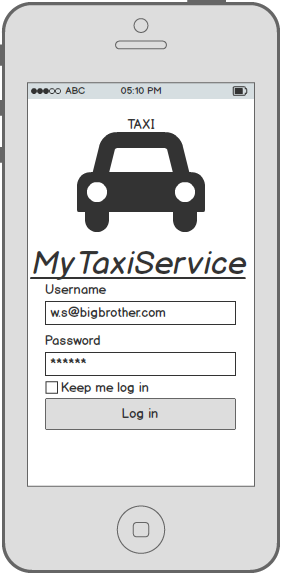
\includegraphics[width=0.6\textwidth, width=3cm]{driverlogin}
				\caption{Driver's log in interface.}
			\end{figure}
			\newpage
		\subsubsection {Driver Work Settings}
		 	The system must provide the driver the acces to his working condition.
		 	\begin{figure}[h!]
				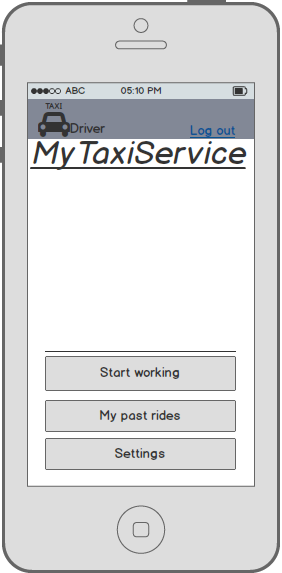
\includegraphics[width=0.6\textwidth, width=3cm]{appdriverlogged}
				\caption{Driver's home page.}
			\end{figure}
			\newpage
		\subsubsection {Driver Ride Acceptance}
			The system must provide the driver to accept or refuse a ride.
		 	\begin{figure}[h!]
				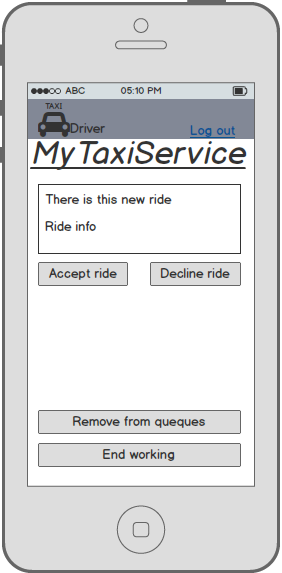
\includegraphics[width=0.6\textwidth, width=3cm]{appdrivernew}
				\caption{Driver's ride information page.}
			\end{figure}
			\newpage
		\subsubsection {Driver Ride Settings}
			The system must provide the driver to know the ride information and eh comand to end it, and be reinserted \askpippo in the queue.
		 	\begin{figure}[h!]
				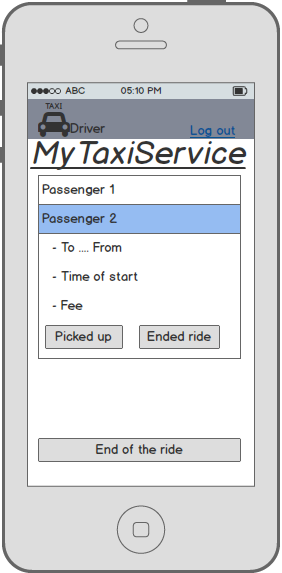
\includegraphics[width=0.6\textwidth, width=3cm]{appdriveron}
				\caption{Driver's ride information page.}
			\end{figure}
			\newpage


\begin{description}

        \item[System Registration and Login] \hfill \\
		The system needs to enable sign up for new users, as well as logins for existing users. Password recovery must also be available.
        \item[User Profile Functions] \hfill \\
		The system must have a profile editing function, where a user can change personal data, such as name as well as their address,
		and also add new payment options. On top of that, the system shall log all the rides a user makes into a database.
		\item[Instant Calls] \hfill \\
		The system must let both registered and unregistered users call a taxi immediately.
		\item[Booking and Sharing] \hfill \\
		The system must let registered users book a ride for a specific date and time. On top of that, there has to be an option to share
		rides with other people who are booking similar routes. Notifications must be sent when a match is found for shared rides. Editing must
		also be available to registered users.
		\item[Worker Functions] \hfill \\
		The system must let registered drivers set their working status. They should therefore let a driver set their status to working or not
		working, and automatically handle their position in queue. A notification system must be put in place to inform a driver of a possible
		ride, as well as the option to accept or refuse a ride.	There should also be a function which lets a driver communicate they ended their
		current ride.
		\item[Taxi Queueing] \hfill \\
		The worker queue must be handled automatically by the system. This includes building a queue dynamically using a FIFO model. The system
		must also move drivers in the queue according to their status:
			\begin{itemize}
				\item A driver set to working shall be added at the end of the queue.
				\item A driver who accepts a ride must be removed from the queue and assigned to a passsenger/s.
				\item A driver refusing a ride should be moved to the end of the queue.
				\item A driver set to not working shall be removed from the queue.
			\end{itemize}

\end{description}
\newpage
\subsection{Functional Requirements}
	After having stated the effective requirements for the system, we can start listing what a user can do.
		\begin{description}
		\item[Unregistered user/Guest] \hfill
			\begin{itemize}
				\item Sign up
				\item Log in
				\item Instant call
			\end{itemize}
		\item[Registered User] \hfill
			\begin{itemize}
				\item Instant call
				\item Change user data, including payment options
				\item View ride history
				\item Advance booking(with sharing options)
				\item Booking modifications
				\item View booking status(including sharing status)
				\item Logout
			\end{itemize}
		\item[Taxi Driver] \hfill
			\begin{itemize}
				\item Set work status
				\item Start a ride
				\item Accept or refuse a ride
				\item Notify end of ride
				\item Logout
			\end{itemize}
		\end{description}
%\endsubsection
\newpage
\subsection{Logical Database Requirements}
	A database should be put in place server-side to handle credential storage, ride booking and ride history. The database responsible for ride history
	shall include where the each ride started and ended, the taxi carrying the passengers and the corresponding driver, and the user/s that made use of the
	taxi(multiple users, up to 4, in case of a shared ride). Note that rides made by unregistered users should also be logged, so drivers may view their own history.
%\endsubsection
\subsection{Design Constraints}

%\endsubsection
\subsection{User Distinction}

%\endsubsection